\documentclass[12pt]{article}
\usepackage[left=2cm, top=2cm, right=2cm, bottom=2cm]{geometry}
\usepackage[utf8]{inputenc}      % accents dans le source
\usepackage[T1]{fontenc}
\usepackage[french]{babel}
\usepackage{graphicx}
\usepackage{graphics}
\usepackage{amsmath}
\usepackage{tikz}
\usepackage{xcolor} 
\usepackage{mathtools}
\usepackage{parskip}
\usepackage{subcaption}
\usepackage[export]{adjustbox}

\title{\vspace{-2cm}\textbf{TP 2 - Ondes progressives ultrasonores}}
\author{MENARD Alexandre - VIEILLEDENT Florent}
% \setlength{\parindent}{1cm}
\date{\vspace{-0.5cm}}

\begin{document}
\maketitle

L'acoustique est l'étude des ondes sonores dans différents milieux. Elle trouve des applications dans le développement des chambres
anéchoïques où l'on cherche à minimiser au maximum les perturbations sonores pour permettre des mesures précises sur le son émis par des appareils par exemple. 
Notre travail ici consistera à caractériser les ondes sonores progressives ultrasonores par observation qualitative. Nous proposerons
deux protocoles pour déterminer la célérité de ces dernières et nous mesurerons les coefficients de transmission et réflexion pour différents matériaux.

\section{Mesure de la célérité du son}
Dans cette partie, nous mesurerons la célérité du son à l'aide de la longueur d'onde et de la fréquence du son émis mais aussi par une seconde méthode basée sur la réflexion de l'onde.

\subsection{Génération et caractérisation d'une onde sonore}
L'émetteur sonore est composé d'un matériau dit piézo-électrique capable de se déformer sous un champ électrique. Ainsi, soumis à un champ électrique
le matériau va se déformer et générer un déplacement du milieu donc une onde sonore. Pour une première approche, nous suivons le protocole
expérimental dans la section \textbf{1.1}. Nous observons alors des signaux ayant [\dots].

On remarque que l'onde ne perd pas en amplitude sur son trajet et que sa forme est semblable à une sinusoïde, nous pourrons donc poser que l'amplitude est constante et que l'énergie est conservée dans l'onde.

Nous passons ensuite l'émetteur en mode "salves courtes" en suivant le protocole de la partie \textbf{1.3.1}. Nous observons alors des signaux de la forme suivante:
\begin{figure}[!htbp]
	\centering
	INSERER SCHEMA
	\hfill
	\caption{Signal émis en salves courtes}
\end{figure}

\subsection{Modèle}
En suppose que l'onde émise est parfaitement sinusoïdale et que la dissipation de l'énergie de l'onde sur la distance est négligeable, l'amplitude $A$ restant donc constante. 
Nous pouvons modéliser la propagation de cette dernière avec $k=\frac{2\pi}{\lambda}$, $\nu$ la fréquence et $\phi$ la phase à l'origine:
\begin{align}
	y(x, t) = A \sin(2\pi\nu t - kx + \phi)
\end{align}

Si deux signaux (émis ou reçus) sont en phase, on a alors en deux positions $x_1$ et $x_2$:
\begin{align*}
	y(x_1, t) = y(x_2, t) & \Rightarrow |x_1 - x_2| = n\lambda
\end{align*}

La célérité de l'onde sera alors donnée par $c = \lambda \nu$. Dans le cas d'une mesure par réflexion, si l'on note $\Delta t$ le temps de trajet de l'onde, et $d$ la distance parcourue, on aura $c = \frac{d}{\Delta t}$

\subsection{Protocole expérimental}
Nous suivrons les protocoles expérimentaux 1 et 2 fournis dans la section \textbf{1.2} pour relever une vingtaine de positions dont 10 avec un seul récepteur en mouvement, et 10 autres
avec un récepteur fixe et un second en mouvement. La vingtaine de mesures permet de "diluer" le bruit de fond qui pourrait être présent au moment de la mesure mais aussi car l'on relève une position
lorsque les deux signaux sont en phase, ce qui est à l'appreciation de l'expérimentateur. On partagera donc les 20 mesures entre 2 expérimentateurs pour limiter une erreur systématique dû à un des expérimentateurs. 
La fiche technique de l'émetteur précise une fréquence émise \textbf{autour} de 40kHz, on prend donc $\nu = 40 \pm 0.2 \text{kHz}$ pour tenir compte de l'absence d'une incertitude précise. 
Les positions des récépteurs et de l'émetteur sont notés $x_{re_1}, x_{re_2}, x_{em}$ et ont des incertitudes associées
$\delta x = 0.1cm$ que l'on détermine par les graduations fournies par le rail gradué. 
Nous utilisons le mode \textit{trigger}
de l'oscilloscope pour stabiliser la forme du signal en synchronisant le balayage horizontal à un certains point du signal et faciliter la lecture de ce dernier.
\begin{figure}[!htbp]
	\centering
	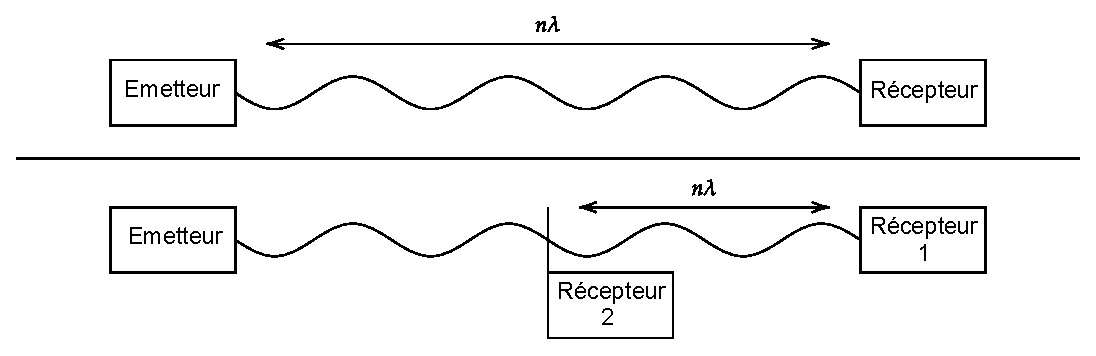
\includegraphics[width=0.6\textwidth]{img/schema}
	\hfill
	\caption{Schéma des deux protocoles 1 et 2}
\end{figure}

\break
\section{Mesure des coefficients de transmission et réflexion}
Dans cette expérience, on détermine le coefficient de réflexion et de transmission de différents écrans. 
\subsection{Modèle}
-Expliquer ce que sont les coeffs (On doit justifier ? Pourquoi au carré? Parler de l'absobtion --> dire qu'on la néglige pour l'instant et on voit plus tard qu'on peut peut être pas)
-Relier l'amplitude en volt et l'amplitude de l'onde? --> je pense pas, mais il demande de justifier notre calcul des coeffs dans le poly je suis pas sûr de ce qu'ils veulent

\subsection{Protocole expérimental}

On place un premier récepteur à côté de l'émetteur et un autre à 20 centimètres. On place l'écran qu'on souhaite étudier entre l'émetteur et le deuxième récepteur, à 10 centimètres. On obtient l'amplitude de l'onde incidente en plaçant un récepteur à l'endroit où on place l'écran, à 10 centimètres en face de l'émetteur. On mesure les amplitudes grâce à un oscilloscope. Les incertitudes sur les amplitudes sont donc données par la précision à laquelle on peut régler l'oscilloscope. 

\begin{figure}[h!]
	\begin{center}
		\includegraphics[scale=0.1]{img/Schéma_Ecran.png}
		\label{Schéma Ecran}
		\caption{(En haut) Schéma du montage expérimentale sans écran. (En bas) Schéma du montage expérimentale avec écran.}
	\end{center}
\end{figure} 

\subsection{Résultats et interprétations}

\break
\section*{Annexes}
\subsection*{Table de données pour la }
\end{document}